% AMBAC full paper（詳細版）第 1 版（2026-11-26）
% 学術論文版レター（../letter/letter_formal.tex）を土台に、第 2 段階（シミュレーション場）の詳細、
% 校正の誤差評価の全体、失敗の記録（docs/13 §13.5）、3 層目の照合の計画（番外編）を加えた版。
% tex は版ごとに別のファイルとして残す（AMBAC_fullpaper_v1.tex, v2, ...）。PDF は AMBAC_fullpaper.pdf に上書きする。
% ビルド: report/fullpaper/ で latexmk -lualatex -jobname=AMBAC_fullpaper AMBAC_fullpaper_v1.tex
\documentclass[paper=a4paper,fontsize=10pt,twocolumn,column_gap=2zw,line_length=24zw,number_of_lines=46,head_space=20mm]{jlreq}
\usepackage{amsmath,amssymb,bm}
\usepackage{graphicx,xcolor}
\usepackage{booktabs,array,multirow,longtable}
\usepackage{tikz}
\usetikzlibrary{arrows.meta,positioning}
\usepackage[hidelinks]{hyperref}
\usepackage{url}
\graphicspath{{./}{../letter/}{../../figures/}}
\newcommand{\repo}{https://github.com/okamasaya/simulation_AMBAC}
\newcommand{\fpversion}{第 1 版（2026 年 11 月 26 日）}
\setlength{\textfloatsep}{8pt plus 2pt minus 2pt}
\setlength{\floatsep}{6pt plus 2pt minus 2pt}
\setlength{\abovecaptionskip}{3pt}
\renewcommand{\arraystretch}{1.08}

\title{\textbf{安価なシミュレーションと校正値は\\フィジカル AI の何を助けるか（詳細版）}\\[0.3em]
\large --- 手足による姿勢制御（AMBAC）を「答えの分かっている試験台」として：\\誤差評価と失敗の記録を含めて ---}
\author{simulation\_AMBAC プロジェクト}
\date{\fpversion}

\begin{document}
\twocolumn[
\begin{@twocolumnfalse}
\maketitle
\vspace{-1.5em}
\begin{center}\begin{minipage}{0.9\textwidth}\small
\textbf{概要}\quad
フィジカル AI（身体を持って実世界で動く AI）の開発は、高価な実機、sim-to-real ギャップ、構造のない探索の難しさ、実機の校正という課題を抱える。
本稿は、実機も GPU を前提とする高精細なシミュレータも使えない条件で、CPU だけで動く安価なシミュレーションがこれらの課題のどこまでに答えられるかを、
手足の運動の反作用で胴体の向きを変える AMBAC（Active Mass Balance Auto Control）を試験台として検討する。
AMBAC は基本式が 1 本で、最適解と理論上界が分かる非ホロノミック系であり、学習・制御・校正の手法を「答え合わせ」できる。
(1) 構造を持たない方策は、ループ運動の効果が振幅の 2 次であるために探索に失敗するが、振動子の構造を与えると理論上界の 98\% に達した。
(2) モデル誤差と外乱の下では、ドメインランダム化で学習した方策の終端誤差は 0.09°で、開ループの最適制御（30.5°）より頑健だったが、推進剤の節約は最適制御が担うべき「最初の判断」に集中していた。
(3) 物理エンジン上に部品表から機体を組み立てる「シミュレーション場」を作り、17 の段階で、組み合わせた形が要求した動きを実現できるか、どの校正値が性能を左右するかを調べた。
(4) 答えを隠した仮想の実機で質量・慣性を推定し、誤差を統計・計算・系統に分けて評価した。微分を使わない推定は偏りが有意でなく（独立な 2 標本 100 回の平均で 0.07\% 以下）、1 試行のばらつきは 1.4〜1.6\% だった。
当初「誤差約 2\%」と見えた偏りの主因は、推定法ではなく\textbf{仮想の実機自身の 1 次の積分法}であり、それが推定しにくい方向（質量・慣性の全体の大きさ）で 2 桁拡大されていた。
関節角も誤差のある測定値として $L=0$ を拘束条件とする当てはめ（素粒子実験の kinematic fit）は、ばらつきを同じ試行で 30\%（95\% 区間 14〜43\%）減らし、推定ごとの誤差を正しく見積もった（pull の標準偏差 1.04）が、推定しにくい方向の系統誤差は $\chi^2$ に現れなかった。
本稿は、成功だけでなく\textbf{うまくいかなかった 13 の試みとその原因を、先行研究で知られた失敗と対応づけて}記録し、
安価なシミュレーションの役割は実機の代わりではなく、\textbf{学習に与える構造・学習と制御の分担・校正の試験動作と測るべき量を、実機の前に絞り込むこと}にあると論じる。
学習は進化戦略に限った事例であり、他の学習法・他の系・実機への一般化は今後の検証課題である。
\end{minipage}\end{center}
\vspace{1em}
\end{@twocolumnfalse}
]

\section{はじめに}

フィジカル AI は、ロボットのように身体を持って実世界で動く AI である。
その開発には、次の課題がよく知られている。
\begin{enumerate}\setlength{\itemsep}{0pt}
\item \textbf{実機が高価}で、試行錯誤のたびに壊すリスクと時間がかかる。
\item \textbf{sim-to-real ギャップ}：シミュレーションで学習した方策が実機で動かない。ドメインランダム化 \cite{tobin2017,peng2018}、アクチュエータのモデル化 \cite{hwangbo2019} などで対処されてきた。
\item \textbf{探索と構造}：報酬だけを与えたモデルフリー学習は、物理の構造を知らないため局所解に陥りやすい。歩行では CPG \cite{ijspeert2008} や軌道生成器 \cite{iscen2018} が構造として用いられる。
\item \textbf{校正（システム同定）}：質量・慣性・摩擦・アクチュエータ特性など、シミュレーションと実機の差を埋める値（校正値）を、どの試験動作で、どの精度で測れるか \cite{atkeson1986,gautier1990}。
\end{enumerate}

大規模な GPU シミュレーション \cite{makoviychuk2021} は (2) を力業で解く有力な道だが、計算資源を持たない研究者・開発者には手が届きにくい。
我々も実機を持たず、高精細なシミュレーションや映像制作には最新世代の GPU が必要とされる状況にある。
そこで本稿は逆の問いを立てる。\textbf{CPU だけで動く安価なシミュレーションは、上の課題のうち何に答えられ、何に答えられないか。}

試験台には AMBAC を選ぶ。AMBAC は、外トルクのない状態で手足の質量を動かし、その反作用で胴体の姿勢を制御する方式である。
宇宙飛行士の自己回転 \cite{kane1970} や落下する猫の空中での立ち直り \cite{kane1969,montgomery1993}、自由浮遊宇宙ロボットの非ホロノミックな経路計画 \cite{nakamura1991} と同じ原理に基づく。
AMBAC を選んだ理由は、(i) 基本式が 1 本で、(ii) 最適解と理論上界を別に計算でき、(iii) 非ホロノミック性という学習にとって本質的な難しさを含むため、
学習・制御・校正の手法を「答え合わせ」できる点にある。

\textbf{本稿の位置づけ}：本稿は、A4 約 5 ページの学術論文版（レター）\cite{letter2026} の詳細版である。
レターの 3 つの課題（第 3〜5 節）に加えて、
第 2 段階の「シミュレーション場」の 17 段階の結果（第 6 節）、校正の誤差評価の全体と本版で行った再評価（第 7 節）、
\textbf{うまくいかなかった試みとその原因}（第 8 節）、そして実物との照合を始めるための最小の実験計画（第 9 節）を収めた。
失敗の記録を本文に含めるのは、先行研究と同じ形で失敗していれば、それ自体が我々の仮説と論理が同じ道筋をたどっている証拠になり、
後発が先行研究に追いつく足場になると考えるからである。

本稿の貢献は次の 5 点である。
(1) 探索の失敗の原因を物理の構造（2 次の効果）として特定し、構造を与えた学習が専門家を上回ることを示す（第 3 節）。
(2) モデル誤差の下で、学習と最適制御の得意・不得意を分ける（第 4 節）。
(3) 部品表から機体を組み立てるシミュレーション場で、組み合わせた形の性能と、性能を左右する校正値を洗い出す（第 5・6 節）。
(4) 答えを隠した仮想の実機で、校正の誤差を統計・計算・系統に分けて評価し、シミュレータ自身が系統誤差の源になることを示す（第 7 節）。
(5) 失敗の記録を先行研究の既知の失敗と対応づけ、誤差評価の手順として整理する（第 8 節）。
すべてのコードと数値は公開している\footnote{\url{\repo}}。課題・役割・結果の対応を図~\ref{fig:overview} に示す。

\begin{figure*}[t]\centering\small
\begin{tikzpicture}[>=Stealth,
  prob/.style={draw,rounded corners,fill=gray!8,text width=3.6cm,align=left,minimum height=1.25cm,font=\footnotesize},
  role/.style={draw,rounded corners,fill=blue!6,text width=4.6cm,align=left,minimum height=1.25cm,font=\footnotesize},
  res/.style={draw,rounded corners,fill=orange!8,text width=5.9cm,align=left,minimum height=1.25cm,font=\footnotesize},
  head/.style={font=\small\bfseries}]
\node[prob] (p1) at (0,0) {探索が構造を知らない\\（局所解・平らな評価）};
\node[prob] (p2) at (0,-1.5) {モデル誤差・外乱\\（sim-to-real ギャップ）};
\node[prob] (p3) at (0,-3.0) {組み合わせた形の性能\\（何が効くか）};
\node[prob] (p4) at (0,-4.5) {実機の校正\\（何を・どう測るか）};
\node[role] (r1) at (4.7,0) {物理の構造から失敗の原因を予測し、\\方策に与える構造を選ぶ};
\node[role] (r2) at (4.7,-1.5) {同じ条件で学習と最適制御を比べ、\\役割の分担を決める};
\node[role] (r3) at (4.7,-3.0) {部品表から機体を組み立て、\\同じ物差しで仕組みを 1 つずつ足す};
\node[role] (r4) at (4.7,-4.5) {答えを隠した仮想の実機で、\\推定の手順と測るべき量を決める};
\node[res] (s1) at (10.8,0) {構造なし：誤差 50〜120°\\振動子の構造：理論上界の 98\%（第 3 節）};
\node[res] (s2) at (10.8,-1.5) {学習：誤差 0.09°（開ループ最適制御 30.5°）\\推進剤の計画は最適制御が有利（第 4 節）};
\node[res] (s3) at (10.8,-3.0) {止めるときの反作用・足元の摩擦の境目・\\荷重分布・サーボの遅れが効く（第 5・6 節）};
\node[res] (s4) at (10.8,-4.5) {拘束つきの当てはめで誤差を自己評価（pull 1.04）。\\積分法が系統誤差の源（第 7 節）。失敗 13 件（第 8 節）};
\node[head,above=1pt of p1] {フィジカル AI の課題};
\node[head,above=1pt of r1] {安価なシミュレーションの役割};
\node[head,above=1pt of s1] {AMBAC での結果};
\foreach \i in {1,2,3,4}{\draw[->,thick] (p\i)--(r\i); \draw[->,thick] (r\i)--(s\i);}
\end{tikzpicture}
\caption{本稿の構成：フィジカル AI の課題と、実機の代わりではない安価なシミュレーションの役割、AMBAC を試験台にした結果の対応。}\label{fig:overview}
\end{figure*}


\section{試験台：AMBAC}

\subsection{基本式と幾何学的位相}
外力のない平面の多体系で、胴体の姿勢角を $\theta$、関節角を $\bm q$ とすると、全角運動量は $L = A(\bm q)\dot\theta + \bm B(\bm q)\cdot\dot{\bm q}$ と書ける。
静止から始めれば $L=0$ なので、
\begin{equation}
\dot\theta = -\bm\Gamma(\bm q)\cdot\dot{\bm q},\qquad \bm\Gamma = \bm B/A
\label{eq:ambac}
\end{equation}
が AMBAC の基本式である。$\bm\Gamma$ は幾何力学の機械的接続 \cite{marsden1992} で、次の性質を持つ。
\begin{itemize}\setlength{\itemsep}{0pt}
\item \textbf{時間を含まない}：回転角は関節の経路だけで決まり、速さによらない。
\item \textbf{関節 1 つでは可逆}：腕を戻すと姿勢も戻る。人間大のモデルで腕 1 本を 180° 振ると、胴体は $-16.04^\circ$ 回り、戻すと元に戻る。
\item \textbf{関節 2 つ以上のループで正味の回転}：関節空間の閉曲線 $C$ を 1 周すると、ストークスの定理より
$\Delta\theta = -\iint_S F\,dq_1dq_2$（$F=\partial_1\Gamma_2-\partial_2\Gamma_1$ は接続の曲率）だけ回る（幾何学的位相）。繰り返せば任意の角度へ回れる。
\end{itemize}
人間大の腕＋脚のモデルでは、1 周あたり $+2.98^\circ$ で、ストークスの定理による値と一致した。
曲率 $F$ の符号と大きさは関節空間の場所で変わるため、\textbf{どこで・どの向きに・どれだけの面積のループを回すか}が、AMBAC の設計変数になる。

\subsection{大きさの効果（二乗三乗則）}
機体を相似に $s$ 倍すると、質量は $s^3$、慣性モーメントは $s^5$ で増え、同じ角加速度に必要な関節トルクは $s^5$ で増える。
一方、アクチュエータの断面に比例して使えるトルクは $s^3$ 程度でしか増えないため、関節の角速度、ひいては AMBAC の旋回の速さは $1/s$ で落ちる。
18 m 級の機体では 90° の旋回に約 2 分かかり、スラスタとの併用が前提になる（第 4 節）。

\subsection{AI の言葉に言い直すと}
AMBAC は「行動（関節の速度）の効果が、行動の\textbf{順序と組み合わせ}でしか現れない」課題である。
正味の回転は入力ベクトル場のリー括弧から生じ、滑らかな時不変フィードバックでは安定化できない（Brockett の定理 \cite{brockett1983}）。
1 回の動きの効果は振幅の 1 次、ループの正味の効果は振幅の 2 次であり、この次数の差が、第 3 節の探索の失敗の原因になる。


\section{課題 1：探索と帰納バイアス}

\textbf{設定}：人間大の腕＋脚のモデル（$L=0$）で、「胴体を目標角まで回せ」とだけ報酬を与え、物理の知識（接続・曲率・ループ）は与えない。
進化戦略（ES）\cite{salimans2017} で次の 3 種類の方策を学習した（第 3・4 節の学習はすべて ES による。他の学習法での再現は第 10 節で論じる）。
\textbf{plain}：観測（姿勢誤差、関節角）→ MLP → 関節角速度。
\textbf{cpg}：plain の観測に周期信号を追加。
\textbf{tg}：振動子が目標関節角のループ（中心・振幅・形）を生成し、その形と位相の速さを学習する（PMTG \cite{iscen2018} と同系統）。
比較として、最適な円ループを回すモデルベース制御（expert）を用いた。

\begin{table}[t]\centering\small
\caption{25 s 後の姿勢誤差（目標角ごと）}\label{tab:learn}
\begin{tabular}{lcccc}\toprule
目標 & plain & cpg & \textbf{tg} & expert \\\midrule
$+90^\circ$ & 61.8° & 61.8° & \textbf{0.2°} & 8.7° \\
$-90^\circ$ & 49.7° & 49.7° & \textbf{0.1°} & 7.9° \\
$+150^\circ$ & 121.8° & 121.8° & \textbf{0.4°} & 21.3° \\\bottomrule
\end{tabular}
\end{table}

\begin{figure*}[t]\centering
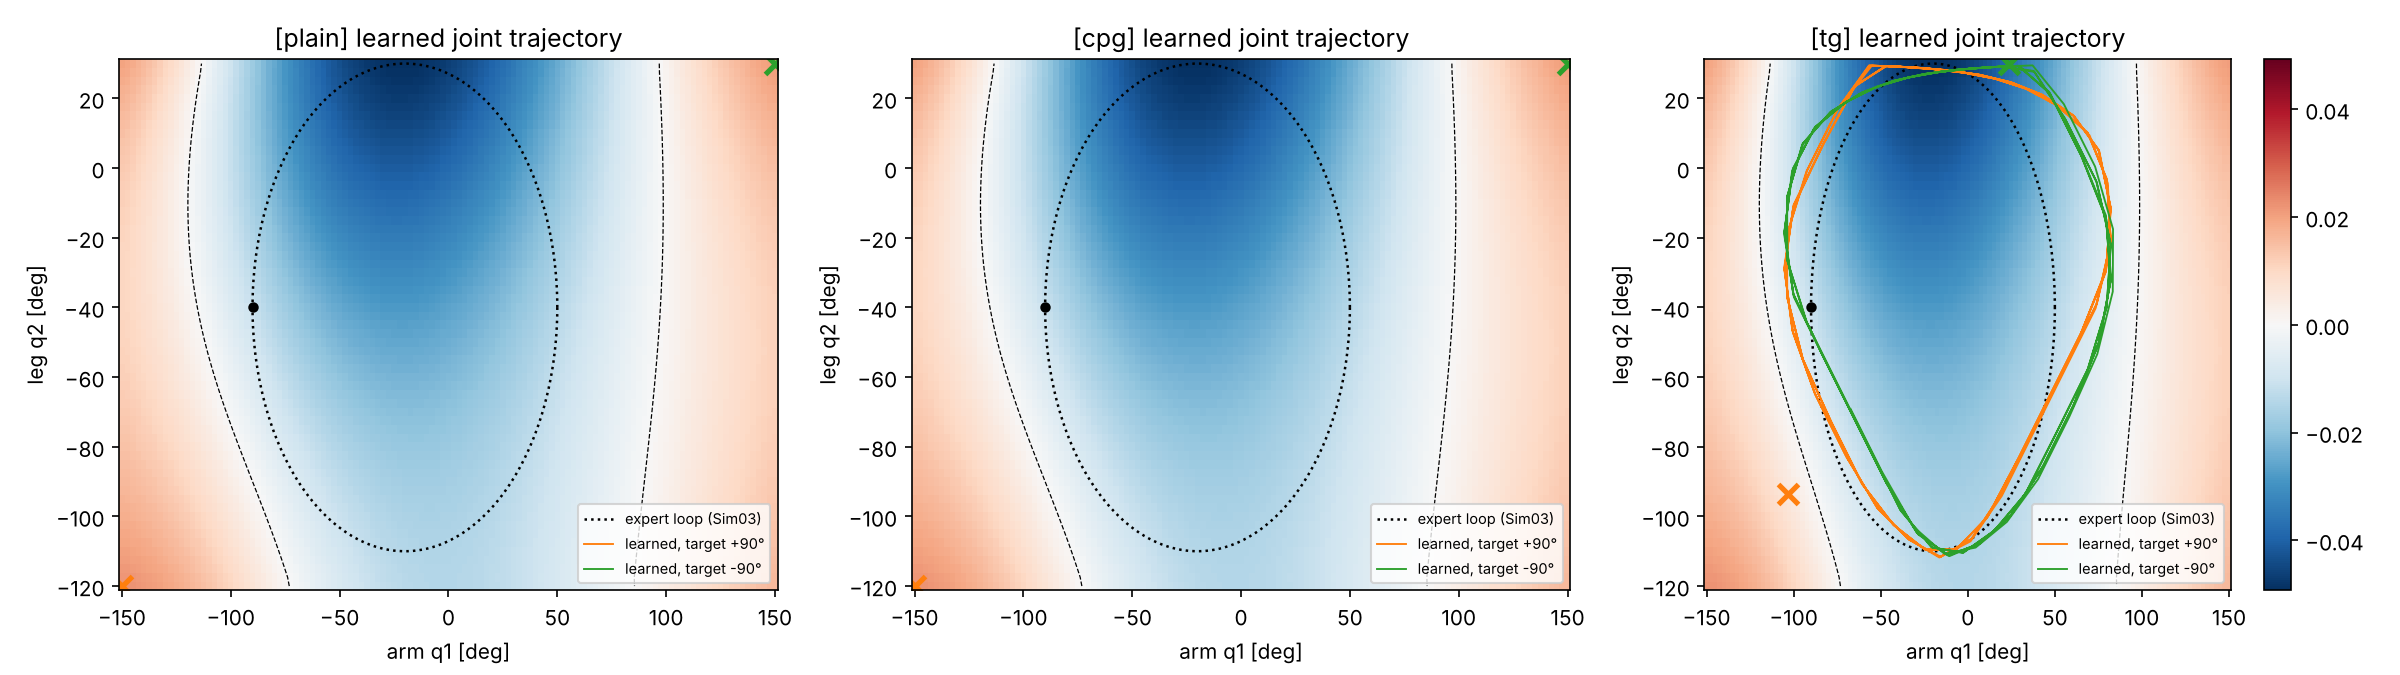
\includegraphics[width=0.86\textwidth]{figs/learn_top.png}
\caption{学習した関節の軌道（色は接続の曲率 $F$）。plain と cpg は手足を可動域の端まで振って止まる局所解（×印）に収束する。
振動子の構造を持つ tg は、曲率が負の領域をほぼ埋めるループを見つけた。点線は人手で設計した最適円ループ。}\label{fig:learn}
\end{figure*}

\textbf{結果}（表~\ref{tab:learn}、図~\ref{fig:learn}）：plain と cpg は、手足を可動域の端まで振って止まる局所解に収束した。
tg は数十イテレーションで解を見つけ、1 周 $+9.34^\circ$ のループを学習した。これは人手で設計した最適円（$+6.70^\circ$）を上回り、可動域内の理論上界（$+9.57^\circ$）の 98\% に達する。
回す向きも曲率の符号と整合し、最後に「揺れの少ない位相で止まる」ことまで覚えて、終端誤差は expert より 1 桁以上小さかった。

\textbf{なぜ構造なしでは失敗するのか}：1 回の動きの効果（可逆な首振り $-\bm\Gamma\cdot\Delta\bm q$）は振幅の 1 次だが、ループの正味の回転（曲率 × 囲んだ面積）は振幅の 2 次（$\propto A_1A_2$）である。
静止に近い方策から探索を始めると、ループを大きくする方向の勾配はほぼ 0 になり、1 次の効果である「端まで振る」が先に最適化される。
これはハイパーパラメータの問題ではなく、課題の物理構造に由来する。周期信号を観測に足すだけ（cpg）では足りず、「ループを描く」という\textbf{形}を方策の構造として与えることが成否を分けた。
plain と cpg の誤差が 3 つの目標で完全に一致するのは、両者が同じ「端まで振る」解に収束したことの表れである。

同じ現象は地上でも現れた（第 6 節、段階 6）。MuJoCo \cite{todorov2012} を評価関数として直接使い、荷物運びの腰と肘の動きを Nelder--Mead 法で最適化したところ、
最初から短い動作時間で探すとどの係数でも転倒して評価が平らになり、探索が進まなかった。
時間を少しずつ短くする継続法で、荷物運びの時間は 65\% 短縮し、「反ってから前に傾く」という人が重い物を持つときの動き（腰の戦略）が再発見された。
\textbf{評価が平らになる領域を、物理の構造から予測し、避ける設計}が、安価なシミュレーションで事前に検討できる。


\section{課題 2：モデル誤差と、学習・最適制御の分担}

\textbf{設定}：18 m 級の機体で、スラスタと AMBAC を併用して 90° の旋回を 60 s で行う。
制御器は周回平均の「平均化モデル」しか知らず、評価には周回内の揺れを含む「位相モデル」を用いる（モデル誤差）。
さらにループ形状の効き（$\times0.7$〜$1.3$）、慣性（$\times0.9$〜$1.1$）、一定の外乱トルクをランダムに変えた 100 例で比べた。
学習方策は観測（平均姿勢の誤差、角運動量、残り時間、ループの位相）からスラスタのトルクとループの周波数を出す MLP で、同じランダムな条件で学習した（ドメインランダム化 \cite{peng2018}）。

\begin{table}[t]\centering\small
\caption{モデル誤差・外乱がある 100 例での比較}\label{tab:robust}
\setlength{\tabcolsep}{4pt}\begin{tabular}{lccc}\toprule
制御器 & 終端誤差 & 残留角速度 & 推進剤 \\
 & 平均（95\%） & [°/s] & [kg] \\\midrule
開ループ最適制御 & 30.5°（68.8°） & 0.90 & \textbf{1.97} \\
MPC & 14.6°（23.3°） & 0.030 & 5.41 \\
MPC＋揺れ補償 & 0.19°（0.69°） & 0.031 & 5.56 \\
学習方策 & \textbf{0.09°（0.10°）} & \textbf{0.002} & 4.92 \\\bottomrule
\end{tabular}
\vspace{1pt}\par\footnotesize 参考：公称モデルでのスラスタのみの最適値は 3.62 kg。
\end{table}

\textbf{結果}（表~\ref{tab:robust}）：線形計画で解いた開ループの最適制御は、推進剤は最小だが、終端誤差が 30° に達した。
平均化モデルの予測自体は正確（平均姿勢 89.6° 対予測 90.0°）で、誤差の原因は止まった位相での揺れだった。
人手で揺れの補償を加えた MPC は誤差 0.19° まで改善したが、学習方策は\textbf{観測に位相を入れただけで}同じことを自力で獲得し、誤差 0.09°、残留回転は MPC の 1/10 だった。
実行時の計算も行列積だけで済む（100 例で 0.1 s 対 LP の再計画で 15〜40 s）。

一方、学習方策の推進剤は、スラスタだけの最適値より多かった。
スラスタで角運動量を一度入れると、止めるときに同じ量の逆噴射が必ず要るため、\textbf{AMBAC が推進剤を節約できるのは「最初にどれだけ噴くか」を決める段階だけ}である。
報酬が終端でしか与えられない学習では、この最初の判断の価値を割り当てにくく（信用割り当ての問題）、学習方策は AMBAC で得をする余地を自ら消していた。

\textbf{示唆}：保存量（角運動量）の収支のように、最適性が明示的な構造で決まる部分は最適制御で計画し、
モデル誤差・外乱・速い揺れの補正は学習で担う、という分担（残差学習 \cite{johannink2019}）が自然である。
第 3 節と合わせると、\textbf{「形」（ループ）は方策の構造として与え、「保存量」は計画で扱う}という、物理の知識と学習の分担の指針が得られる。


\section{シミュレーション場：方法}

ここからが、現在進めている第 2 段階である。
PC 上に、障害物のない「試験場」と、段差・坂・低摩擦面・低重力などを置ける「ステージ」を用意し、物理エンジン MuJoCo（CPU のみ）で機体を動かす。
目的は、\textbf{組み合わせた形で、要求した動きを実現できるか}を、校正値と制御を含めて確かめることである。進め方は次の 4 つである。

\begin{enumerate}\setlength{\itemsep}{0pt}
\item \textbf{3 層の照合}：第 1 段階の Python の基準モデル（答えが分かっている）と MuJoCo を照合してから、MuJoCo でしかできない試験に進む。将来の実機を 3 層目とする（第 9 節）。
\item \textbf{部品表から機体を組み立てる}（アセンブル）：台車・腰・肩（1〜3 軸）・肘・履帯・ばね・円盤などを JSON の部品として組み合わせる。
\item \textbf{段階的に組み込む}：基準の試験に仕組みを 1 つずつ足し、同じ物差しで比べる。
\item \textbf{目で確かめる}：数値とグラフに加えて、動画で動きを見る。履板の食い込み、床を突き抜けた腕、電源を切った後に動く腕は、動画で見つけた。
\end{enumerate}

\textbf{シミュレータ自体の照合}：基準モデルと MuJoCo を同じ関節の動きで比べた。
腕 1 本の往復で $-16.0356^\circ$ 対 $-16.0356^\circ$、腕＋脚のループ 1 周で $+2.963^\circ$ 対 $+2.970^\circ$ と一致し、角運動量の保存は $10^{-6}$ 程度だった（この照合は積分法 RK4 による）。
ゲーム用の物理エンジンは安定化のための減衰などで角運動量が厳密には保存されないことがあり、1 周数度の幾何学的位相は埋もれうる。
\textbf{答えの分かっている試験に合格させること自体が、シミュレータの校正}になる。
ただし第 7 節で見るように、この照合に合格した後でも、部品表から組み立てた機体の既定の積分法（implicitfast、1 次）が、校正の試験では系統誤差の源になった。
照合は「どの積分法・時間刻みで」合格したかまで含めて記録する必要がある。

\begin{figure*}[t]\centering
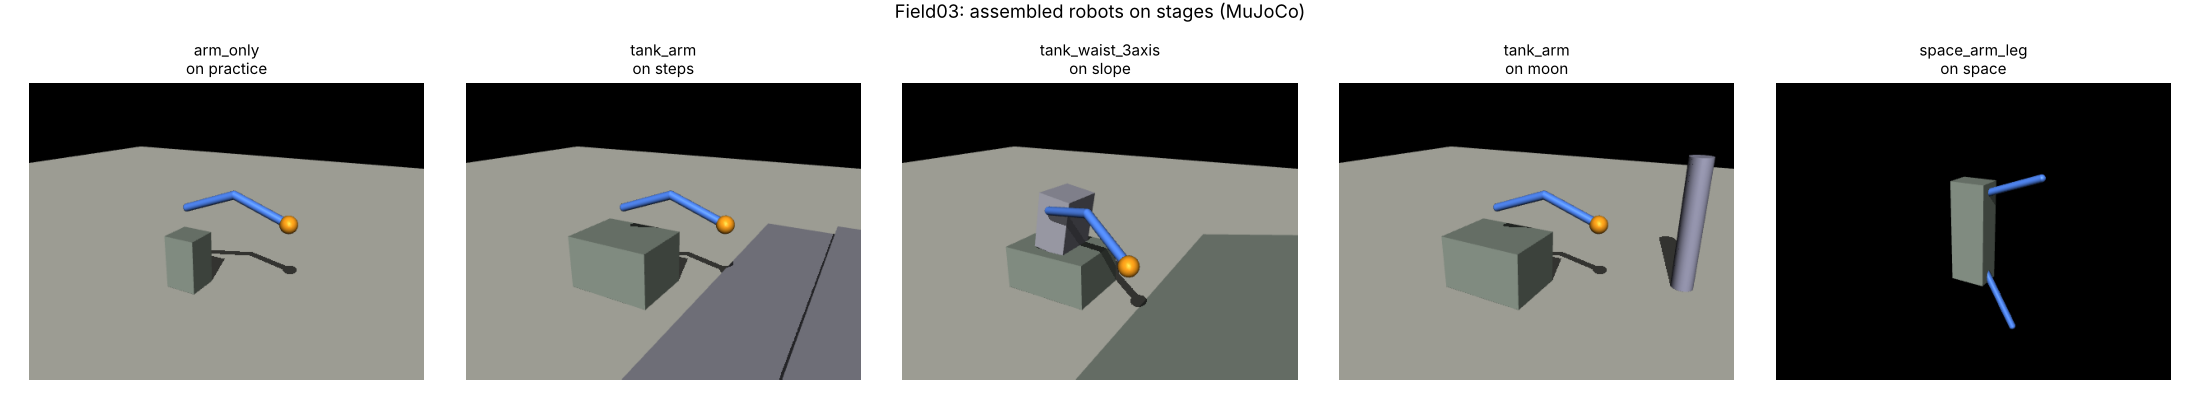
\includegraphics[width=0.92\textwidth]{field/field03_gallery.png}
\caption{部品表（JSON）から組み立てた機体の例（段階 3）。台車・腰・肩・肘・履帯などの部品を組み合わせ、手作りのモデルと同じ結果になることを確かめてから、ステージでの試験に使った。}\label{fig:gallery}
\end{figure*}


\section{シミュレーション場：結果}

\begin{table*}[t]\centering\small
\caption{シミュレーション場の段階ごとの成果}\label{tab:stages}
\setlength{\tabcolsep}{4pt}
\begin{tabular}{clp{0.62\textwidth}}\toprule
段階 & 内容 & 主な結果 \\\midrule
1 & 宇宙の試験場 & 基準モデル（腕の往復 $-16.04^\circ$、ループ 1 周 $+2.98^\circ$）と一致。シミュレータの妥当性を確認 \\
2 & 地上の試験場 & 転倒の始まりが基準モデルと一致。旋回で台車が浮く条件（第 1 段階の前提が崩れる場合）を発見 \\
3 & アセンブル & 部品表から機体を組み立て、手作りのモデルと一致 \\
4 & 仮想の実機で校正 & 答えを隠した機体の質量・慣性を推定。誤差の評価と kinematic fit は第 7 節 \\
5 & 性能表・校正データ & 重力だけが違うステージではフルード則が 1\% の精度で成立、氷では外れる。CSV・JSON・Excel を出力 \\
6 & 腰の戦略の最適化 & 荷物運びを最大 65\% 短縮。「反ってから前に傾く」動きを再発見。トルクは 3 倍に \\
7 & モーターの定格 & 荷物を支えるトルク（地球 130・月 22 N·m）が実現の境目 \\
8・10 & 段差・坂（履帯） & 坂は摩擦の限界（31°）どおり。段差は長い履帯で 2 倍（0.15 → 0.30 m）。短い機体は後ろに転倒 \\
9 & 二本脚と戦車型 & 二本脚は腰なしでは荷物を運べない。腰ありでも戦車型より約 3 割遅い \\
11 & 2 本の履帯の旋回 & スキッドステアの基準モデルと 0〜11\% で一致。長い履帯は旋回に 1.6 倍の力。荷重分布を一様と仮定すると 3 割ずれる \\
12 & 腕の振りと向き & 腕の非対称な往復で車体を回せる（摩擦の非対称性による地上版 AMBAC） \\
13 & 腕の反作用への対策 & 車体が回るのは腕を「止めるとき」。しなり（ばね）は逆効果、逆回転するおもりは有効 \\
14 & 止め方・流体ブレーキ & トルクを境目より下に抑えて止めると、車体を回さずに 1.2〜1.35 s で振れる。流体の種類で得意な場面が逆 \\
15 & 機能を分けた組み合わせ & 動かす＝モーター、止める・保持する＝MR ブレーキで 1.18 s、行き過ぎ 0.2°、電源なしでも保持 \\
16 & 繰り返しの発熱と劣化 & 先に限界に達するのはモーター。MR で止めると続けられる頻度が 2 倍。寿命は約 150 万回 \\
17 & 3 軸の肩＋肘 & モーター＋MR が、車体を乱さない方式で最速。電源を切っても腕が落ちない（2 mm） \\\bottomrule
\end{tabular}
\end{table*}

段階ごとの成果を表~\ref{tab:stages} にまとめる。フィジカル AI の観点から重要な結果は次の 3 つである。

\textbf{(1) 地上の反作用と足元の摩擦の境目}：
宇宙では腕の反作用はすべて機体の回転になるが、地上では、\textbf{足元の摩擦が車体を回し始めるトルク（この機体で約 260 N·m）までは、反作用を摩擦が吸収する}。
境目を超えた分だけが、車体の回転や滑りとして現れる。車体を乱すのは主に腕を\textbf{止めるとき}で、位置サーボの遅れ（最大 17°）が急ブレーキを生み、この境目を超えさせていた（図~\ref{fig:reaction}）。
反作用の山の高さだけでなく、境目を超えている時間（力積）が効くため、しなり（ばね）は山を下げても境目より下まで下げられなければ逆効果だった。
一方で、摩擦の非対称性を使えば、腕を「速く振ってゆっくり戻す」往復で車体の向きを変えられる。宇宙の AMBAC（幾何学的位相）とは別の仕組みの、地上版の AMBAC である。

\begin{figure*}[t]\centering
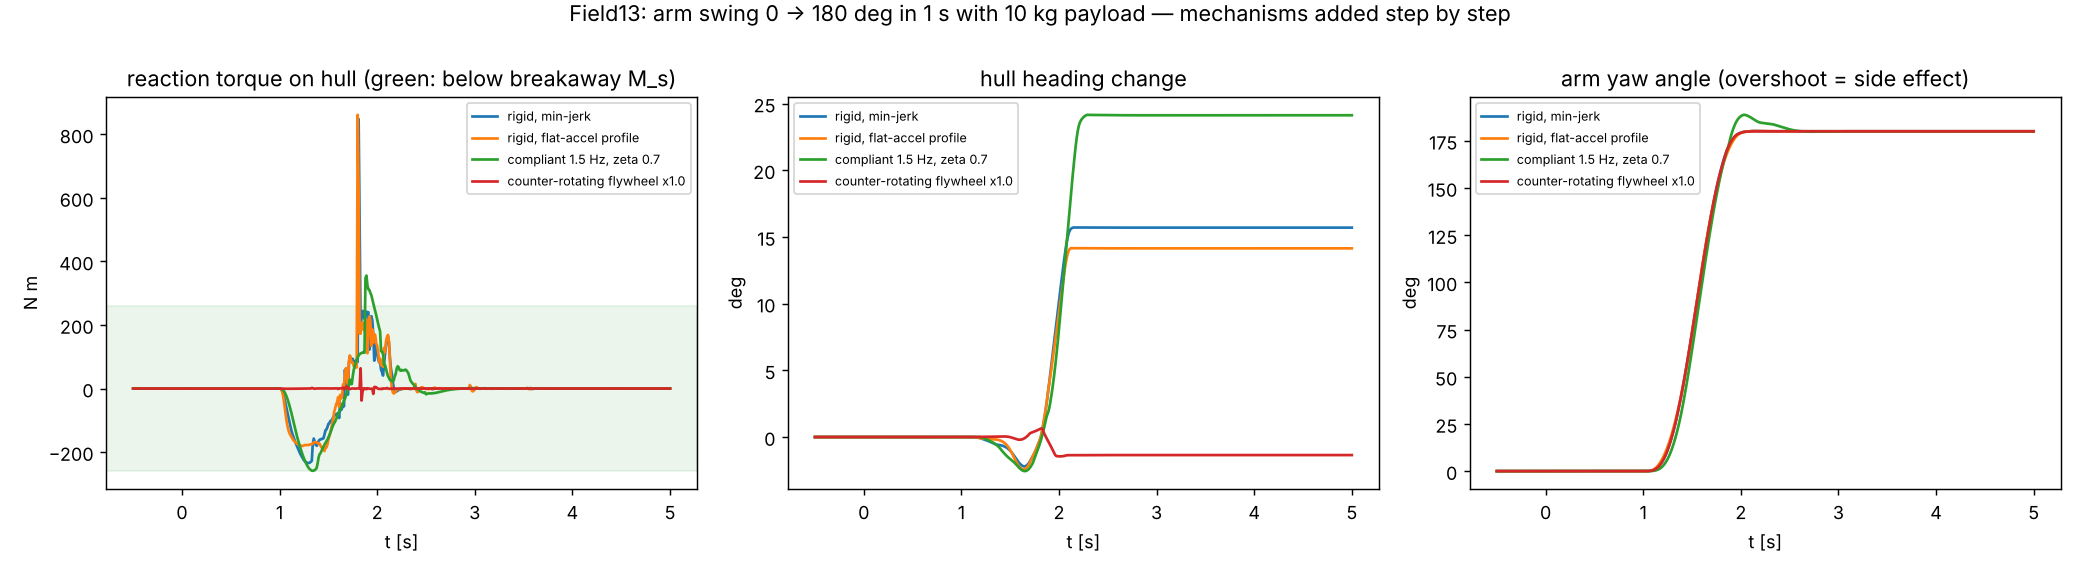
\includegraphics[width=0.92\textwidth]{field/field13_reaction.png}
\caption{腕の反作用と車体の回転（段階 13）。車体が回るのは、腕を止めるときの反作用が足元の摩擦の境目を超えた区間で、位置サーボの遅れがその急ブレーキを生む。しなり（ばね）は山を下げるが、境目を超える時間（力積）を減らせず逆効果になる。}\label{fig:reaction}
\end{figure*}

\textbf{(2) 機能を分ける}：止め方を変える（トルクを境目より下に抑えて一定に止める）だけで、追加の部品なしに車体を乱さず速く動けた。
さらに、動かすのはモーター、止める・保持するのは MR 流体のブレーキ、と機能ごとに部品を分けて上の制御で使い分けると、速さ・精度・省エネ・電源なしの保持が同時に向上した（段階 15・17）。
人の体の筋肉（動かす）・腱（しなる）・靭帯や関節の摩擦（保持する）と同じ考え方である。
MR は熱で効きが落ち、使うほど劣化するが、劣化は熱に変えたエネルギーの総量（LDE）で予測でき、定期的な流体の交換で受け止められる（段階 16。温度係数と寿命は製品のデータで要確認）。

\textbf{(3) 性能を左右する校正値}：組み立てた機体の試験から、表~\ref{tab:calibvals} の量が性能を大きく左右することが分かった。
これらは、\textbf{モデルに含めた誤差源の中で}、実機で何を先に測るべきかの候補を与える。
重力だけが違うステージでは荷物運びの最短時間がフルード則（$\propto\sqrt{\text{大きさ}/g}$）で 1\% の精度で移せたが、氷では外れ（予測 1.35 s 対 2.22 s）、制約が転倒から滑りに変わった。摩擦は重力のスケーリングとは別の校正値である。

\begin{table}[t]\centering\small
\caption{性能を左右すると分かった校正値}\label{tab:calibvals}
\setlength{\tabcolsep}{3pt}
\begin{tabular}{p{0.42\linewidth}p{0.38\linewidth}c}\toprule
校正値 & 何を決めるか & 段階 \\\midrule
質量・慣性（腕・脚・胴体） & AMBAC の効き & 4 \\
足元の摩擦の境目と荷重移動による変化 & 腕の作業で車体が乱れるか & 12〜14 \\
接地の荷重分布 & 旋回の速さ（一様の仮定で 3 割ずれる） & 11 \\
関節の慣性（姿勢で変わる） & 止める計算 & 17 \\
サーボの遅れ（ゲイン） & 軌道の崩れ、急ブレーキ & 13 \\
摩擦（重力とは別） & 氷でのフルード則の破れ & 5 \\
モーターの銅損・熱抵抗、MR の温度係数・寿命 & 続けて動かせる頻度、保守の周期 & 7・16 \\\bottomrule
\end{tabular}
\end{table}

\textbf{シミュレーション場を作るうえでの教訓}：
MuJoCo は計算が発散すると状態を初期化するため、発散が「止まった」結果に紛れる。走行の試験では発散を検出して記録するようにした。
また、腕の動き（秒）と温度（分〜時間）のように時間の桁が違う現象は、前者を MuJoCo、後者を熱の簡単なモデルで扱い、組み合わせた。


\section{課題 3：校正値を実機の前に設計する}

\subsection{答えを隠した仮想の実機}
実機の代わりに、腕・脚の質量（$\pm15\%$）と胴体の慣性（$\pm10\%$）を乱数でずらした機体を作り、正解を推定する側に隠した（総質量 76 kg は既知とする）。
曲率マップの異なる場所に置いた 6 種類のループを 1 周ずつ回し、ジャイロ（雑音 0.2°/s、一定のバイアス最大 $\pm0.2$°/s）とエンコーダ（雑音 0.05°）を 100 Hz で模擬記録して、推定結果を正解と比べた。
推定法は、(a) 1 周ごとの正味の回転だけ、(b) 周回中の角速度の波形（関節角を微分して $\dot{\bm q}$ を求める）、
(b$'$) 式~(\ref{eq:ambac}) が時間を含まないことを利用し、0.1 s の区間ごとの回転量を $-\int\bm\Gamma\cdot d\bm q$ と比べる（微分なし）、
(c) (b) に関節トルクの情報を加える、の 4 つである。いずれもジャイロのバイアスを同時に推定する。

\begin{figure*}[t]\centering
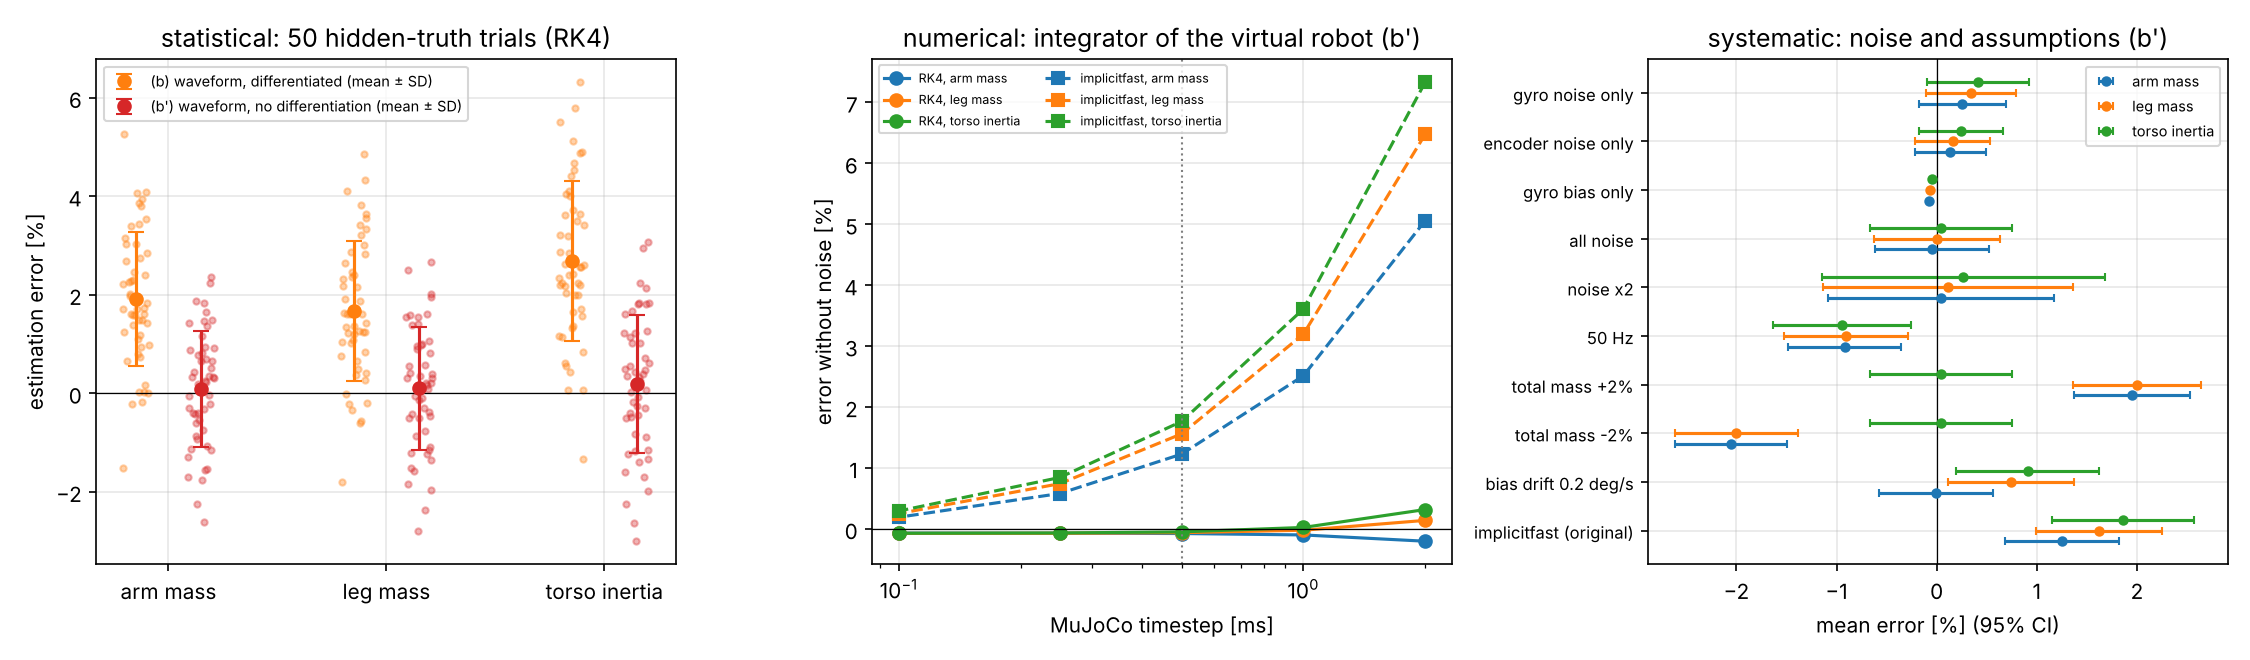
\includegraphics[width=0.84\textwidth]{figs/error_budget.png}
\caption{答えを隠した仮想の実機による校正の誤差評価。左：統計誤差（正解と雑音を変えた 50 回の試行、点は各試行、誤差棒は平均 $\pm$ 標準偏差）。
中：計算誤差（雑音なしの推定誤差と、仮想の実機の時間刻み・積分法。点線は既定の 0.5 ms）。
右：系統誤差（雑音の種類と推定側の仮定を 1 つずつ変えたときの平均の偏り、誤差棒は 20 通りの雑音による 95\% 信頼区間）。}\label{fig:calib}
\end{figure*}

\subsection{誤差の評価：統計・計算・系統}

\begin{table}[t]\centering\small
\caption{推定誤差（平均 $\pm$ 標準偏差 [\%]、腕 / 脚 / 慣性）。(a)(b) は field04b の 50 回。(b$'$) は独立な 2 標本（field04b・04c）をまとめた 100 回で、平均の 95\% 信頼区間の半幅は 0.27〜0.32\%。}\label{tab:calib}
\footnotesize\setlength{\tabcolsep}{2pt}
\resizebox{\linewidth}{!}{\begin{tabular}{lccc}\toprule
推定の方法 & 腕 & 脚 & 慣性 \\\midrule
(a) 正味の回転 & $-7\pm28$ & $+103\pm145$ & $+16\pm42$ \\
(b) 微分 & $+1.9\pm1.4$ & $+1.7\pm1.4$ & $+2.7\pm1.6$ \\
(b$'$) 微分なし & $\bm{-0.01\pm1.37}$ & $\bm{+0.00\pm1.45}$ & $\bm{+0.07\pm1.63}$ \\
kinematic fit（第 7.4 節） & $\bm{-0.01\pm1.09}$ & $\bm{+0.04\pm1.14}$ & $\bm{+0.04\pm1.29}$ \\\bottomrule
\end{tabular}}
\end{table}

\begin{table}[t]\centering\small
\caption{(b$'$) の誤差の内訳 [\%]（腕 / 脚 / 慣性）}\label{tab:budget}
\setlength{\tabcolsep}{3pt}
\begin{tabular}{p{0.52\linewidth}c}\toprule
誤差の種類 & 大きさ \\\midrule
\multicolumn{2}{l}{\textbf{統計誤差}} \\
\quad 1 試行の標準偏差（100 回） & 1.37 / 1.45 / 1.63 \\
\quad \quad 標本 04b / 04c（各 50 回） & 1.2--1.4 / 1.5--1.8 \\
\quad 100 回の平均の 95\% 信頼区間 & $\pm$0.27 / 0.28 / 0.32 \\
\multicolumn{2}{l}{\textbf{計算誤差}（雑音なし）} \\
\quad 時間刻み 0.5→0.1 ms（RK4） & 0.02 以下 \\
\quad 最適化の収束条件 & 0.001 以下 \\
\quad 推定式の離散化・モデル差 & $-0.07$ \\
\quad 積分法 implicitfast（0.5 ms） & \textbf{+1.2 / +1.6 / +1.8} \\
\multicolumn{2}{l}{\textbf{系統誤差}（20 通りの雑音の平均）} \\
\quad 雑音による偏り（全雑音） & $-0.05$ / 0.00 / +0.05 \\
\quad 総質量の仮定 $\pm2\%$ & $\pm2.0$ / $\pm2.0$ / 0.0 \\
\quad バイアスのドリフト 0.2°/s & 0.0 / +0.7 / +0.9 \\
\quad サンプリング 50 Hz & $-0.9$ / $-0.9$ / $-0.9$ \\
\quad サンプリング 200 Hz & 0.0 \\\bottomrule
\end{tabular}
\end{table}

\textbf{統計誤差}（図~\ref{fig:calib} 左、表~\ref{tab:calib}）：ループ 1 周の正味の回転だけ (a) では、脚の質量を推定できなかった。
波形を使う (b) と (b$'$) の 1 試行のばらつきは主にジャイロの雑音による（ジャイロの雑音だけで 1.0\%）。
(b$'$) の平均は 0.1\% 以下で、95\% 信頼区間が 0 を含み、偏りは統計的に有意でない。

\textbf{本版での再評価：ばらつきの見積もりそのものの揺らぎ}：
レター \cite{letter2026} では (b$'$) の 1 試行のばらつきを、誤差評価のための 50 回（field04b）から 1.2〜1.4\% と報告した。
ところが、kinematic fit の評価（field04c）でも、同じ条件（RK4、0.5 ms、同じ雑音とバイアスの設定）で別の乱数の 50 回について (b$'$) を計算しており、そちらでは 1.5〜1.8\% だった。
2 つの標本の分散の比は 1.71〜1.74 で、ブートストラップの 95\% 区間は 1.01〜2.88、比が 1 を下回る割合は 2\% だった（約 2$\sigma$ の食い違い）。
外れ値によるものではなく（中央絶対偏差でも同じ傾向）、誤差の大きさとバイアスの大きさにも相関はなかった（相関係数 0.03〜0.06）。
条件の違いは見つからず、最も単純な解釈は、50 回の標本では 1 試行の標準偏差そのものが 10\% 程度揺らぎ、その揺らぎの端どうしを比べた、というものである。
そこで本稿では 2 標本をまとめた 100 回の値（1.37 / 1.45 / 1.63\%）を採用し、レターの「1.2〜1.4\%」は過小評価側だったと訂正する（\texttt{sims/field04d\_dispersion\_pool.py}）。
これは、後述の F4（5 回の試行での過小評価）と同じ種類の誤りが、50 回でも小さな形で残りうることを示す。

\textbf{系統誤差}（図~\ref{fig:calib} 右、表~\ref{tab:budget}）：(b) は +1.7〜2.7\% 偏り、信頼区間は 0 を含まない。偏りはエンコーダの雑音だけでも生じ、サンプリングを 200 Hz に上げると +3〜7\% に増え、雑音を 2 倍にしても増えた。
雑音の入った関節角を微分して推定式に入れると偏る errors-in-variables の典型であり、微分を避けた (b$'$) にはこの偏りがない。
推定側の仮定では、既知とした総質量の誤差が腕・脚の質量にそのまま 1:1 で移り、バイアスのドリフトとサンプリングの粗さが 1\% 弱の偏りを生んだ。

\subsection{計算誤差：シミュレータ自身が系統誤差の源になる}
当初、仮想の実機は部品表から組み立てた MuJoCo のモデルを既定の積分法 implicitfast（1 次）で計算しており、元の 5 回の試行では (b$'$) の誤差が 5 回ともプラス側にそろっていた（平均 +1.6〜2.3\%、ばらつき 0.5\%）。
「誤差約 2\%」の大部分は、偶然のばらつきではなく系統的な偏りだった。
雑音を除いても +1.2〜1.8\% の偏りが残り、偏りは時間刻みに比例した（2 ms で +5〜7\%、0.5 ms で +1.2〜1.8\%、0.1 ms で +0.2〜0.3\%）。
原因は、1 次の積分法で角運動量 $L=0$ がわずかに保たれないことにある。式~(\ref{eq:ambac}) からのずれは姿勢の角速度の 0.02\% 程度にすぎないが、
推定はこのずれを、次に述べる推定しにくい方向（全体の大きさ）に沿って吸収するため、パラメータでは 2 桁大きい偏りになる。
第 1 段階の手作りの機体は RK4 で計算していたため、段階 1 の照合ではこの問題は現れなかった。
積分法を RK4 にすると、0.5 ms でも雑音なしの誤差は 0.08\% 以下になった。
\textbf{答えを隠した仮想の実機で校正を設計するとき、仮想の実機自身の数値誤差が、推定しにくい方向で拡大されて系統誤差として現れる}。
これを見逃すと、推定法の限界や前処理の問題と取り違える（我々も当初は、偏りの原因を前処理だけに帰していた。第 8 節 F5）。

\textbf{推定しにくい方向}：腕・脚の質量と胴体の慣性が\textbf{そろって同じ割合で増減する方向}が推定しにくい（特異値がほかの方向の約 1/60、推定の相関係数 0.99 以上）。
式~(\ref{eq:ambac}) は質量・慣性の「比」しか含まないため、姿勢の波形だけでは全体の大きさが決まらない。
これはマニピュレータの同定で知られる「推定可能なパラメータの組み合わせ」\cite{gautier1990} と同じ構造で、
総質量の誤差が質量の推定に 1:1 で移ることも、この構造の表れである。\textbf{絶対値を決めるには、総質量の正確な計量か、関節トルクなどの力の情報が要る}。
ただし力の情報を関節角の 2 回の微分と組み合わせると（推定法 (c)）、上と同じ理由で偏る（元の条件の 5 回の試行で、誤差は 4〜5\% に悪化した）ため、速度・加速度を直接測るセンサーとの組み合わせが必要になる。

\subsection{拘束条件つきの当てはめによる誤差の自己評価}
実機では正解が分からないため、校正値そのものに加えて「その値をどこまで信じてよいか」を、1 回の校正から示せる必要がある。
そこで、素粒子実験の kinematic fit \cite{avery1998} の考え方を校正に持ち込んだ。
関節角も誤差のある測定値として、その誤差の範囲で動かし、角運動量 $L=0$ を拘束条件として厳密に満たすように、真の関節角の列 $\bm Q$・パラメータ $\bm p$・ジャイロのバイアス $b$ をまとめて当てはめる。
{\small\begin{equation}
\chi^2=\sum_i\frac{\|\bm Q_i-\bm q_{m,i}\|^2}{\sigma_q^2}+\sum_i\frac{\bigl(\omega_{m,i}-b+\bm\Gamma(\bm Q_i;\bm p)\cdot\dot{\bm Q}_i\bigr)^2}{\sigma_\omega^2}
\label{eq:kinfit}
\end{equation}}
$\dot{\bm Q}_i$ は当てはめた $\bm Q$ の中心差分で、雑音の入った測定値を微分しないため、(b) のような偏りは生じない。
未知数は約 5200 個だが、ヤコビアンが疎なので、CPU で 1 回 50 s 程度で解ける。
得られた共分散から、推定ごとの誤差 $\sigma$ と、当てはまりの良さ $\chi^2$ が得られる。

\begin{figure*}[t]\centering
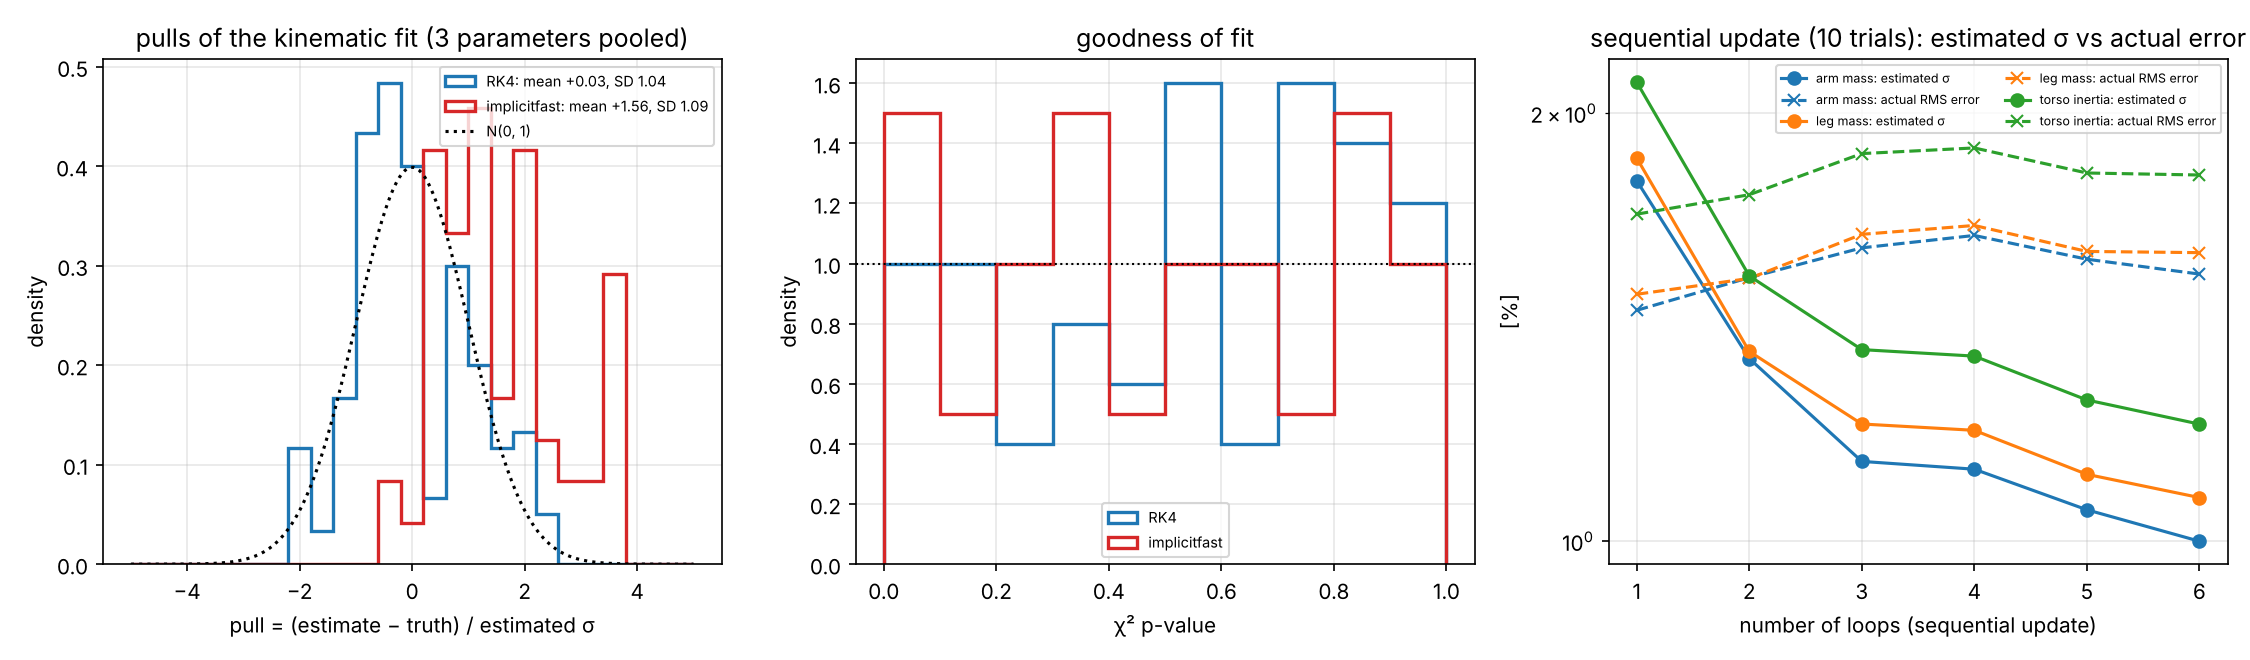
\includegraphics[width=0.84\textwidth]{figs/kinfit.png}
\caption{拘束条件つきの当てはめ（式~(\ref{eq:kinfit})）の自己評価。左：pull $=(\text{推定}-\text{正解})/\sigma$ の分布（3 つのパラメータをまとめた）。RK4 の仮想の実機（50 回）では $N(0,1)$ に一致し、積分法の系統誤差を含む implicitfast（20 回）では $+1.6\sigma$ ずれる。
中：$\chi^2$ の p 値。どちらも一様で、系統誤差は $\chi^2$ に現れない。右：ループを 1 本ずつ加える逐次更新での、推定した $\sigma$（実線）と実際の誤差の二乗平均（破線、10 回）。}\label{fig:kinfit}
\end{figure*}

\begin{table}[t]\centering\small
\caption{kinematic fit の自己評価（腕 / 脚 / 慣性）}\label{tab:kinfit}
\footnotesize\setlength{\tabcolsep}{2pt}
\resizebox{\linewidth}{!}{\begin{tabular}{lcc}\toprule
 & RK4（50 回） & implicitfast（20 回） \\\midrule
誤差の平均 [\%] & $-0.01$ / $+0.04$ / $+0.04$ & $+1.5$ / $+1.8$ / $+2.1$ \\
誤差の標準偏差 [\%] & 1.09 / 1.14 / 1.29 & 1.09 / 1.18 / 1.34 \\
推定した $\sigma$ の平均 [\%] & 1.04 / 1.11 / 1.25 & 1.07 / 1.15 / 1.29 \\
pull の平均 & $+0.01$〜$0.05$ & $+1.4$〜$1.6$ \\
pull の標準偏差 & 1.04〜1.05 & 1.10〜1.11 \\
$|\text{pull}|<1$ の割合 & 66〜68\% & 30〜40\% \\
$\chi^2/\text{ndf}$ & $0.997\pm0.032$ & $1.003\pm0.034$ \\
相関係数 & 0.989〜0.999 & 0.989〜0.999 \\\bottomrule
\end{tabular}}
\end{table}

結果を図~\ref{fig:kinfit} と表~\ref{tab:kinfit} に示す。RK4 の仮想の実機での 50 回の試行で、推定は偏らず（平均 0.04\% 以下）、ばらつきは 1.1〜1.3\% だった。
同じ 50 回の試行で計算した (b$'$) と比べると、標準偏差の比は 0.70（ブートストラップの 95\% 区間 0.57〜0.87）で、\textbf{ばらつきは約 3 割小さい}。
この比較は同じデータに対する対応のある比較なので、前節で見た標本間の揺らぎの影響を受けない（別の標本の (b$'$) と比べると、減り方は 2 割程度に見える）。
\textbf{推定ごとの誤差 $\sigma$ は正しく見積もられ}、pull の平均は 0.01〜0.05、標準偏差は 1.04〜1.05、$|\text{pull}|<1$ の割合は 66〜68\% で、$\chi^2/\text{ndf}=0.997\pm0.032$ だった。

ループを 1 本ずつ加え、前の推定値と共分散を事前情報として当てはめ直す逐次更新（カルマンフィルタと同じ形で、素粒子実験の飛跡の当てはめ \cite{fruhwirth1987} でも用いられる）では、
$\sigma$ はループを加えるごとに 1.8\% から 1.0\% へ縮み、最終値は一括の当てはめと 0.23\% 以内で一致した。
なお、逐次更新を試した 10 回では実際の誤差の二乗平均（1.5\%）が $\sigma$（1.0\%）より大きく見えたが、同じ 10 回の一括の当てはめも 1.55\% で、この 10 回がたまたま誤差の大きい試行だった（F10）。結論は 50 回の pull で出す。

一方、積分法の系統誤差を含む仮想の実機では、pull は $+1.4$〜$1.6\sigma$ ずれたが、\textbf{$\chi^2$ の p 値は一様のままで、当てはまりの良さからは検出できなかった}。
3 つのパラメータの推定の相関係数が 0.99 以上あり、ずれが推定しにくい方向に吸収されるためである。
拘束条件つきの当てはめは誤差の自己評価を与えるが、推定しにくい方向の系統誤差は、正解の分かっている照合など独立な検証と組み合わせて評価し続ける必要がある。

\subsection{誤差評価から学んだこと}
\begin{enumerate}\setlength{\itemsep}{0pt}
\item \textbf{仮想の実機（シミュレータ）自身が系統誤差の源になる。} 保存則など答えの分かっている量で、仮想の実機の数値設定を先に検証する。
\item \textbf{推定しにくい方向は、小さな誤差を大きく拡大し、しかも $\chi^2$ に現れない。} 相関行列と pull を見る。
\item \textbf{誤差の原因を一度決めつけると、取り違える。} 原因は 1 つずつ切り分けて確かめる。
\item \textbf{誤差の見積もりにも誤差がある。} 少数試行のばらつきは過小にも過大にも出るので、独立な標本どうしを比べ、まとめた値と区間で報告する。
\item \textbf{拘束条件つきの当てはめは、推定値とその誤差を同時に与え、逐次更新できる}。フィジカル AI の校正の枠組みとして有望である。
\end{enumerate}


\section{うまくいかなかったこと}

本節では、成功した結果だけでなく、うまくいかなかった試みとその理由を、先行研究や既知の事柄と対応づけて記録する（表~\ref{tab:fail}・\ref{tab:failidx}）。
先行研究と同じ形で失敗していれば、それは我々の仮説と論理が同じ道筋をたどっている証拠になる。

\begin{table*}[t]\centering\footnotesize
\caption{校正の誤差評価と論文化（2026 年 11 月 22〜26 日）でうまくいかなかったこと}\label{tab:fail}
\setlength{\tabcolsep}{3pt}
\begin{tabular}{cp{0.17\textwidth}p{0.19\textwidth}p{0.27\textwidth}p{0.27\textwidth}}\toprule
\# & 試みたこと & うまくいかなかったこと & 原因 & 先行研究・既知の事柄との対応 \\\midrule
F1 & 正味の回転だけで推定 (a) & 脚の質量が決まらない（$+103\pm145\%$） & 正味の回転は 6 個の数しか与えず、3 つのパラメータとバイアスを分けるには情報が足りない & 同定には十分に励起する入力と観測が要る（persistent excitation）。マニピュレータの励起軌道の設計と同じ \\
F2 & 関節角を微分して推定 (b) & +1.7〜2.7\% の有意な偏り。サンプリングを上げると +3〜7\% & 雑音の入った説明変数の微分を回帰に入れると偏る。微分で雑音が増幅される & errors-in-variables の偏り。総最小二乗法や、測定値自体を当てはめる方法（kinematic fit）が対策 \\
F3 & (b) に関節トルクを加える (c) & かえって悪化（4〜5\%） & 加速度を関節角の 2 回の微分で求めるため、F2 がさらに強く出る & 慣性パラメータ同定で加速度の推定が誤差の主因になること \cite{atkeson1986} \\
F4 & 5 回の試行でばらつきを見積もる & 0.5\% と過小評価（50 回では 1.2〜1.8\%） & 試行回数が少なく、偏りが支配的で、ばらつきが偏りに隠れていた & 少数試行での誤差の過小評価。素粒子実験で toy MC を多数回まわして pull を確かめる理由 \\
F5 & 「(b$'$) の偏りの原因は前処理」と結論 & \textbf{誤り}。主因は仮想の実機の積分法 & 雑音・積分法・時間刻みを 1 つずつ変える切り分けをせず、もっともらしい説明で止めた & 系統誤差は原因を 1 つずつ変えて確かめる（素粒子実験の系統誤差の評価の手順） \\
F6 & 組み立てた機体（implicitfast、0.5 ms）を仮想の実機にする & 雑音がなくても +1.2〜1.8\% 偏る（時間刻みに比例） & 1 次の積分法で $L=0$ がわずかに保たれず、そのずれが推定しにくい方向で 2 桁拡大される & 保存則を守らない積分法のドリフト（シンプレクティック積分法の動機）。ゲーム用物理エンジンの角運動量の扱いと同じ問題 \\
F7 & kinematic fit の $\chi^2$ で系統誤差を検出 & pull +1.5$\sigma$ の偏りが $\chi^2$ に現れない & 相関 0.99 以上で、ずれが推定しにくい方向に吸収される & 推定できないパラメータの組み合わせ（base parameters \cite{gautier1990}）。$\chi^2$ の良さは系統誤差がないことを保証しない \\
F8 & 絶対値を姿勢の波形だけで決める & 総質量の仮定の誤差が 1:1 で移る & 式~(\ref{eq:ambac}) が質量・慣性の比しか含まない & F7 と同じ構造。外部の計量か力の情報が必要 \\
F9 & kinematic fit を関数評価 200 回で解く & 上限で打ち切り（収束の保証なし） & 約 5200 個の未知数の収束が遅い & 大規模な当てはめでは収束の判定と反復の上限を確かめる。2000 回で収束を確認 \\
F10 & 逐次更新の 10 回で $\sigma$ と実際の誤差を比べる & 実際の誤差 1.5\% が $\sigma$ 1.0\% より大きく見えた & この 10 回がたまたま誤差の大きい試行（一括の当てはめも 1.55\%） & 少数試行の比較は誤解を生む（F4 と同じ）。結論は 50 回の pull で出す \\
F11 & レター論文に SF 考証を混ぜる & 「技術的な主張のノイズ」と指摘された & 読者と論証の種類が違う内容を 1 本にした & 学術論文と解説・考証の役割分担。2 本に分けて解決 \\
F12 & 画面のないクラウドで MuJoCo を描画付きで動かす & 描画ライブラリがなく起動しない & 環境に osmesa・egl がない & 計算だけなら描画を切って動く \\
F13 & 50 回の試行で (b$'$) のばらつきを 1.2〜1.4\% と報告（レター） & 同じ条件の別の 50 回では 1.5〜1.8\%（分散の比 1.7、約 2$\sigma$） & 50 回でも標準偏差の推定は 10\% 程度揺らぐ。1 つの標本だけで報告した & 誤差の誤差。独立な標本を比べ、まとめた値と区間で報告する（本版で訂正、第 7.2 節） \\\bottomrule
\end{tabular}
\end{table*}

\begin{table}[t]\centering\footnotesize
\caption{これまでの段階の主な失敗（索引）}\label{tab:failidx}
\setlength{\tabcolsep}{2pt}
\begin{tabular}{lp{0.74\linewidth}}\toprule
段階 & うまくいかなかったこと（原因・対応） \\\midrule
Sim05 A & 構造のない方策が端まで振る局所解に収束（効果が振幅の 2 次、Brockett の定理と同じ構造。第 3 節） \\
Sim05 C & 学習方策が推進剤を多く使い、AMBAC の得を自ら消した（信用割り当て。第 4 節） \\
Sim06 & 関節の拘束の不具合（修正後に最短時間 1.00 → 1.03 s） \\
段階 2 & 第 1 段階の旋回モデルが浮き上がり・転倒を見落としていた \\
段階 5 & 氷のステージでフルード則が外れる（摩擦は別の校正値） \\
段階 6 & 最初から短い時間で最適化すると評価が平らになり探索が進まない（継続法で解決） \\
段階 8・10 & 転輪の列の近似で段の角が挟まる、地面を柔らかくすると計算が発散する \\
段階 9 & 二本脚では肘の補正が効かなかった（局所解の可能性） \\
段階 13 & しなりは反作用の山を下げても逆効果。逆回転するおもりは 0.6 s で横倒し \\\bottomrule
\end{tabular}
\end{table}

\textbf{失敗の分類}：13 件は、おおむね次の 3 つに分けられる。
\begin{itemize}\setlength{\itemsep}{0pt}
\item \textbf{情報の不足と推定しにくい方向}（F1・F7・F8）：系の構造（式~(\ref{eq:ambac}) が比しか含まない）から、事前に予測できた失敗である。マニピュレータの同定の先行研究 \cite{gautier1990} と同じ形をしている。
\item \textbf{測定値の微分}（F2・F3）：errors-in-variables という古典的な落とし穴で、拘束条件つきの当てはめで解消した。
\item \textbf{誤差の見積もり方そのもの}（F4・F5・F9・F10・F13）：数値計算や推定法ではなく、\textbf{評価の手順}の失敗である。少数の試行、1 つの標本、切り分けの省略、収束の未確認はいずれも、素粒子実験の解析で手順として防がれている。
\end{itemize}
3 つ目の種類が最も多いことは、安価なシミュレーションで校正を設計するとき、ボトルネックが計算資源ではなく\textbf{評価の手順}にあることを示している。
F6 はこれらにまたがり、シミュレータの数値誤差（計算）が推定しにくい方向（構造）で拡大され、それを前処理のせいと取り違えた（手順）。


\section{3 層目の照合に向けた最小の実験}

ここまでの照合は、基準モデルと MuJoCo の 2 層で、どちらも「剛体はこう動くはずだ」という同じ仮定の上に立っている。
仮定そのものが現実に合っているかは、3 層目の実物と比べるしかない。
実機を持たない条件で始められる最小の実験として、\textbf{1 m のアルミアングル（20 × 20 × 2.0 mm、約 204 g）とスマートフォン 2 台の内蔵 IMU} による剛体の検証を計画している（本稿の時点で未実施）。
記録には、センサーの生データを CSV で書き出せるアプリ phyphox \cite{phyphox} を用いる。

\textbf{実験 A（実体振り子）}：棒の端から $h=0.02$ m の支点で小さく揺らし、周期 $T_0=2\pi\sqrt{I/(Mgd)}$ から支点まわりの慣性モーメント $I$ を求め、部品（棒と端末 2 台）から計算した値と比べる。
端末は 1 台約 144 g で棒より重く、センサーではなく\textbf{剛体の大部分}になるため、部品表から組み立てた 1 つの剛体として扱う（アセンブルの最小の実物版）。
予測値は、棒だけで $T_0=1.623$ s、端末を 0.30 m と 0.90 m に付けて 1.700 s、0.48 m と 0.95 m に付けて 1.738 s である（$g=9.80$ m/s²）。
構成を変えても周期は 5\% 程度しか変わらないため、周期は 0.1\% の精度で測る必要がある。

\textbf{実験 B（回転）}：棒を水平に回し、剛体であれば 2 台の角速度は等しく（比 1.000）、向心加速度は回転軸からの距離に比例する（比 $r_2/r_1=3.00$）ことを確かめる。
$a_c$ 対 $\omega^2$ の傾きから求めた距離はメジャーで測った位置からずれるはずで、そのずれは端末内の\textbf{IMU の取り付け位置}という校正値になる。
これを、第 7.4 節と同じ考え方で、距離とセンサーのバイアスを同時に当てはめて求める。

\begin{table}[t]\centering\small
\caption{実験 A の周期の誤差の見積もり（計画）}\label{tab:bangai}
\setlength{\tabcolsep}{3pt}
\begin{tabular}{lp{0.5\linewidth}p{0.27\linewidth}}\toprule
種類 & 原因 & 周期への影響 \\\midrule
統計 & 零点の時刻（約 100 Hz、20 周期） & 約 0.05\% \\
系統 & 質量の計量（$\pm1$ g） & 約 0.1\% \\
系統 & 端末の位置（$\pm1$ mm） & 約 0.07\% \\
系統 & 支点の位置と穴のガタ（$\pm1$ mm） & 約 0.1\% \\
系統 & 振幅の補正（10° で +0.19\%） & 補正後 0.01\% \\
系統 & 支点の摩擦・空気抵抗 & 減衰から見積もる \\
系統 & 棒のたわみ（剛体の仮定） & 実験 B で確かめる \\
系統 & 重力加速度（地点の値） & 0.01\% 以下 \\
計算 & 積分法と時間刻み & RK4、0.1 / 0.5 ms で比較 \\\bottomrule
\end{tabular}
\end{table}

\textbf{比べ方}：(1) 部品表に棒と端末 2 台を書き、(2) MuJoCo（RK4）で同じ動きをさせ、(3) シミュレータの中に端末と同じ位置・同じサンプリングの仮想の IMU を置き、
(4) 実測とシミュレーションに同じ解析をかけ、(5) 差を誤差で割った pull で判断する。誤差は第 7 節と同じく統計・計算・系統に分けて見積もる（表~\ref{tab:bangai}）。
この実験で見たいのは、剛体の仮定がどこまで成り立つか（速く回したときのたわみ）、シミュレータの誤差と測定の誤差のどちらが大きいか、IMU の校正値を拘束条件つきの当てはめで求められるか、の 3 点である。
その先には、回転椅子に座って棒を手足の代わりに振り、胸に付けた端末で胴体の向きを記録して、式~(\ref{eq:ambac}) とループ 1 周の幾何学的位相を実物で確かめる実験を考えている。
椅子の軸の摩擦は、第 6 節の「足元の摩擦の境目」に当たる。


\section{考察}

\textbf{安価なシミュレーションに答えられること}：
本稿の課題で、シミュレーションは「実機の挙動の予測」ではなく、
\textbf{(1) 学習に与えるべき構造、(2) 学習と制御の分担、(3) 組み合わせた形で効く仕組みと校正値、(4) 校正の試験動作と測るべき量とその誤差}を決めるために使われた。
いずれも、答えの分かっている試験台があるから判断できた。
大規模な GPU シミュレーションとドメインランダム化が「誤差の範囲を広く覆う」方向だとすると、本稿の方向は「どこに誤差があり、何を測ればよいか」を絞る方向であり、両者は補完的になりうる。ただし、これは本稿の事例に基づく仮説であり、両者を同じ課題で比べた検証は行っていない。

\textbf{誤差評価の手順が差を生む}：第 8 節の失敗の多くは、計算資源ではなく評価の手順に由来した。
答えの分かっている照合、原因を 1 つずつ変える切り分け、多数回の試行による pull の確認、独立な標本どうしの比較は、いずれも CPU だけで実行でき、
しかも「誤差約 2\%」の正体（シミュレータの積分法）や、ばらつきの過小評価（F4・F13）を明らかにした。
資源の限られた立場では、\textbf{計算の量ではなく評価の厳密さで、結果の信頼性を上げる}ことが現実的な戦略になる。

\textbf{一般化の射程}：第 3 節の失敗の原因（正味の効果が入力の 2 次、すなわちリー括弧から生じる）は AMBAC に固有ではなく、
車両の縦列駐車に代表される非ホロノミック系、自由浮遊宇宙ロボット \cite{nakamura1991}、ヘビ型・遊泳型の移動など、形状の周期運動で全体を動かす系に共通する。
これらの系では正弦波入力による操舵 \cite{murray1993} が古典的な解法であり、振動子の構造が有効だったことと整合する。
したがって「構造なしの探索は 2 次の効果の前で停滞し、周期運動の構造で解消する」という仮説は、この系の族に対して検証可能な形で立てられる。
第 7 節の「推定しにくい方向で数値誤差が拡大され、$\chi^2$ に現れない」という構造も、パラメータの一部の組み合わせしか観測できない同定問題一般に現れうる。
一方、接触の細部、アクチュエータの非線形、柔軟体のように、誤差の主因がモデルの外にある課題には、本稿の枠組みは直接は届かない。

\textbf{答えられないこと}：PC の上だけでは sim-to-real ギャップそのものは確かめられない。
仮想の実機で絞り込めるのは、モデルに含めたパラメータについて、推定しやすい方向・しにくい方向と、手順上の落とし穴までである。
モデルに入れていない現象（接触の細部、モーターの非線形、部品のたわみ）は再現されず、\textbf{実機で初めて効いてくる未知の誤差源の優先順位は決められない}。
第 6 節のアクチュエータ・MR 流体・熱の数値は仮定の部品の値に基づき、流体ブレーキは速さとトルクの関係を式で与えた理想化したモデルである。

\textbf{学習手法の限定}：本稿の学習はすべて ES による。構造を与える効果が ES に特有のものか、PPO や SAC などの勾配に基づく強化学習を含むモデルフリー学習一般に成り立つかは、本稿の結果からは判断できない。
勾配に基づく手法では探索の初期の方策のばらつきが異なるため、2 次の効果による停滞の程度も変わりうる。同じ試験台で複数の学習法を比べることが、本稿の主張を強めるための最優先の課題である。


\section{今後の目標}

\begin{enumerate}\setlength{\itemsep}{0pt}
\item \textbf{3 層目の照合}：第 9 節の剛体と IMU の実験を行い、シミュレータの剛体の仮定と IMU の校正値を実物で確かめる。その後、安価なサーボのアーム 1 台で、仮想の実機で設計した校正手順を確認する。
\item \textbf{拘束条件つきの当てはめの拡張}：サーボの遅れ・摩擦の校正値を加えて地上の機体（段階 12〜17）へ広げ、総質量の計量や関節トルクのように推定しにくい方向を外から決める情報を拘束として加えて、$\chi^2$ で系統誤差を検出できるかを試す。
投球のような「速度差のある運動の連鎖」を、段ごとの拘束条件の連鎖として当てはめる（粒子の崩壊の連鎖の当てはめとの対応）ことも検討する。
\item \textbf{学習法と系の一般化}：同じ試験台での PPO・SAC との比較と、他の非ホロノミック系（正弦波操舵の古典例など）での構造仮説の検証。
\item \textbf{ハイブリッド制御}：計画を最適制御、実行時の補正を学習方策が担う制御の実装。
\item \textbf{誰でも使えるシミュレータへ}：部品表から機体を組み立て、性能表と校正データを CSV・JSON で書き出すまでをまとめてパッケージとして公開し、校正データを公開して機械学習による推定と物理モデルによる推定を同じデータで比べられるようにする。
\end{enumerate}


\section{まとめ}

実機も高精細なシミュレータも持たない条件で、CPU だけで動く安価なシミュレーションがフィジカル AI の課題にどこまで答えられるかを、AMBAC を試験台に検討した。
構造のない学習の失敗を物理の 2 次の効果として説明し、振動子の構造を与えた学習が理論上界の 98\% に達すること、
モデル誤差の下では学習が頑健だが保存量の計画は最適制御が担うべきこと、
部品表から組み立てた機体の試験で、止めるときの反作用・足元の摩擦の境目・荷重分布・サーボの遅れが性能を左右する校正値になること、
答えを隠した仮想の実機で、校正の誤差を統計・計算・系統に分けて評価し、拘束条件つきの当てはめで推定ごとの誤差を正しく見積もれること、
ただし仮想の実機自身の数値誤差が系統誤差の源になり、それは当てはまりの良さに現れないことを示した。
さらに、うまくいかなかった 13 の試みを先行研究の既知の失敗と対応づけ、その多くが計算資源ではなく評価の手順に由来することを示した。
いずれも ES を用いた単一の系での事例であり、一般化と実物での確認は今後の検証による。
安価なシミュレーションは実機の代わりではなく、\textbf{実機に何を持ち込むべきかを決める道具}として、計算資源の限られた研究者にも開かれている。

\appendix
\section{再現の手順と対応するファイル}
\small
すべてリポジトリ\footnote{\url{\repo}} の相対パスである。画面のない環境では \texttt{MUJOCO\_GL=disable} で実行する。
\begin{itemize}\setlength{\itemsep}{0pt}
\item 第 3・4 節：\texttt{sims/sim05*.py}（学習と制御の比較）。詳しい記録は \texttt{docs/05\_physical\_ai.md}。
\item 第 5・6 節：\texttt{sims/field*.py}（段階 1〜17）、図は \texttt{figures/field/}。記録は \texttt{docs/11}・\texttt{docs/12}。
\item 第 7 節：\texttt{sims/field04b\_error\_budget.py}（誤差の内訳）、\texttt{sims/field04c\_kinfit.py}（kinematic fit、4 並列で約 30 分）、
\texttt{sims/field04d\_dispersion\_pool.py}（本版の再評価、既存の出力の再解析で数秒）。数値は \texttt{data/field04b\_summary.txt}、\texttt{data/field04c\_summary.txt}、\texttt{data/field04d\_summary.txt}。
\item 第 8 節：\texttt{docs/13\_error\_evaluation\_kinfit.md} の 13.5 節。
\item 第 9 節：計画の詳細と理論値は解説記事の原稿 \texttt{articles/ambac-bangai-bar-iphone-imu.md}（未実施、測定値は空欄）。
\end{itemize}

\section{改版の記録}
\small
\begin{description}\setlength{\itemsep}{0pt}
\item[第 1 版（2026-11-26）] 学術論文版レター \cite{letter2026} を土台に作成。
第 2 段階のシミュレーション場の方法と 17 段階の結果（第 5・6 節）、校正の誤差評価の全体と kinematic fit の表（第 7 節）、
失敗の記録（第 8 節、docs/13 §13.5 の F1〜F12 と段階ごとの索引に、本版の再評価で見つけた F13 を追加）、3 層目の照合の実験計画（第 9 節）を加えた。
レターの (b$'$) の 1 試行のばらつき「1.2〜1.4\%」を、独立な 2 標本 100 回の「1.37 / 1.45 / 1.63\%」に訂正し、kinematic fit による改善「約 3 割」を同じ試行での対応のある比較（0.70、95\% 区間 0.57〜0.87）として示し直した。
同時期に、内容を一般の技術者向けに書き直した解説記事（日本語・英語）の原稿をリポジトリの \texttt{articles/}・\texttt{books/}・\texttt{docs/Dev\_Comminuty/} に用意した（未公開）。
\end{description}

\begin{thebibliography}{99}\footnotesize\setlength{\itemsep}{0pt}
\bibitem{letter2026} simulation\_AMBAC プロジェクト, 「安価なシミュレーションと校正値はフィジカル AI の何を助けるか --- 手足による姿勢制御（AMBAC）を『答えの分かっている試験台』として ---」, 学術論文版（レター）, 2026（\texttt{report/letter/letter\_formal.tex}）.
\bibitem{tobin2017} J.~Tobin et al., ``Domain randomization for transferring deep neural networks from simulation to the real world,'' \textit{IROS}, 2017.
\bibitem{peng2018} X.~B.~Peng, M.~Andrychowicz, W.~Zaremba, P.~Abbeel, ``Sim-to-real transfer of robotic control with dynamics randomization,'' \textit{ICRA}, 2018.
\bibitem{hwangbo2019} J.~Hwangbo et al., ``Learning agile and dynamic motor skills for legged robots,'' \textit{Science Robotics}, 4(26), 2019.
\bibitem{ijspeert2008} A.~J.~Ijspeert, ``Central pattern generators for locomotion control in animals and robots: a review,'' \textit{Neural Networks}, 21(4), 642--653, 2008.
\bibitem{iscen2018} A.~Iscen et al., ``Policies modulating trajectory generators,'' \textit{CoRL}, PMLR 87, 916--926, 2018.
\bibitem{atkeson1986} C.~G.~Atkeson, C.~H.~An, J.~M.~Hollerbach, ``Estimation of inertial parameters of manipulator loads and links,'' \textit{IJRR}, 5(3), 101--119, 1986.
\bibitem{gautier1990} M.~Gautier, W.~Khalil, ``Direct calculation of minimum set of inertial parameters of serial robots,'' \textit{IEEE Trans. Robotics and Automation}, 6(3), 368--373, 1990.
\bibitem{makoviychuk2021} V.~Makoviychuk et al., ``Isaac Gym: High performance GPU-based physics simulation for robot learning,'' \textit{NeurIPS Datasets and Benchmarks}, 2021.
\bibitem{kane1970} T.~R.~Kane, M.~P.~Scher, ``Human self-rotation by means of limb movements,'' \textit{J. Biomechanics}, 3(1), 39--49, 1970.
\bibitem{kane1969} T.~R.~Kane, M.~P.~Scher, ``A dynamical explanation of the falling cat phenomenon,'' \textit{Int. J. Solids and Structures}, 5(7), 663--670, 1969.
\bibitem{montgomery1993} R.~Montgomery, ``Gauge theory of the falling cat,'' in \textit{Dynamics and Control of Mechanical Systems}, Fields Inst. Commun. 1, AMS, 1993.
\bibitem{marsden1992} J.~E.~Marsden, \textit{Lectures on Mechanics}, Cambridge University Press, 1992.
\bibitem{brockett1983} R.~W.~Brockett, ``Asymptotic stability and feedback stabilization,'' in \textit{Differential Geometric Control Theory}, Birkhäuser, 181--191, 1983.
\bibitem{salimans2017} T.~Salimans et al., ``Evolution strategies as a scalable alternative to reinforcement learning,'' arXiv:1703.03864, 2017.
\bibitem{todorov2012} E.~Todorov, T.~Erez, Y.~Tassa, ``MuJoCo: A physics engine for model-based control,'' \textit{IROS}, 2012.
\bibitem{nakamura1991} Y.~Nakamura, R.~Mukherjee, ``Nonholonomic path planning of space robots via a bidirectional approach,'' \textit{IEEE Trans. Robotics and Automation}, 7(4), 500--514, 1991.
\bibitem{murray1993} R.~M.~Murray, S.~S.~Sastry, ``Nonholonomic motion planning: steering using sinusoids,'' \textit{IEEE Trans. Automatic Control}, 38(5), 700--716, 1993.
\bibitem{avery1998} P.~Avery, ``Applied fitting theory VI: Formulas for kinematic fitting,'' CLEO Note CBX 98-37, 1998.
\bibitem{fruhwirth1987} R.~Frühwirth, ``Application of Kalman filtering to track and vertex fitting,'' \textit{Nucl. Instrum. Methods A}, 262, 444--450, 1987.
\bibitem{johannink2019} T.~Johannink et al., ``Residual reinforcement learning for robot control,'' \textit{ICRA}, 2019.
\bibitem{phyphox} S.~Staacks, S.~Hütz, H.~Heinke, C.~Stampfer, ``Advanced tools for smartphone-based experiments: phyphox,'' \textit{Physics Education}, 53(4), 045009, 2018.
\end{thebibliography}

\end{document}
